\section{Introduction}
\label{Introduction}

In recent years, Deep Reinforcement Learning (RL) has succeeded at solving complex tasks, from defeating humans in board games \citep{AlphaZero} to complex control problems \citep{sim2real, ppo}. It relies on different learning algorithms (e.g., A2C - \citep{A2C}, PPO - \citep{ppo}). These methods aim at discovering a policy that maximizes the expected (discounted) cumulative reward received by an agent given a particular environment. %If existing techniques work quite well in this setting, a larger amount of research is now dedicated to the generalization in RL setting. 
%Indeed, in many practical RL applications, considering that the environment at train time and the environment at test time are similar is unrealistic. As an example, when learning to drive a car, a student will learn to drive using a particular car, and under specific weather conditions. But at test time, we expect this driver to be able to generalize to any new car, new roads and new weather conditions. This setting makes reinforcement learning more difficult since the algorithm now has to learn a policy \textbf{that generalizes} to unseen environments.
If existing techniques work quite well in the classical setting, considering that the environment at train time and the environment at test time are similar is unrealistic in many practical applications. As an example, when learning to drive a car, a student  learns to drive using a particular car, and under specific weather conditions. But at test time, we expect the driver to be able to generalize to any new car, new roads, and new weather conditions. It is critical to consider the generalization issue where one of the challenges is to learn a policy that generalizes and adapts itself to \textbf{unseen environments}.

Different techniques have been proposed in the literature (Section \ref{sec:relatedwork}) to automatically adapt the learned policy to the test environment. In the very large majority of works, the model has access to multiple training environments (meta-RL setting). Therefore, the training algorithm can identify which variations (or invariants) may occur at test time and how to adapt quickly to similar variations. But this setting may still be unrealistic for concrete applications: for instance, it supposes that the student will learn to drive on multiple cars before getting their driving license. 

\begin{figure}[t]
    \begin{subfigure}{.5\textwidth}
        \begin{center}
        \includegraphics[width=0.8\linewidth]{images/space2.png}
        \end{center}
        \vspace{-0.1cm}
        \caption{The figure represents the parameter space. The red  (resp. blue) region is the space of good policies over the training (resp. testing) environment. A single learned policy (red point) may be inefficient for the test environment and has to be adapted (e.g., fine-tuning) to become good at test-time (blue point). Instead of learning a single policy, we learn a convex sub-space (the pentagon) delimited by anchor policies (red stars) that aims at capturing a large set of good policies. Then the adaptation is just made by sampling policies in this subspace, keeping the best one (blue star).}
        \label{fig:3}
    \end{subfigure}
    \hspace{0.2cm}
        \begin{subfigure}{.5\textwidth}
        \includegraphics[width=1.0\textwidth]{images/k-shot_ant.png}
        \caption{Qualitative example of k-shot adaptation on a modified Ant environment (20\% of observations masked). 5 policies (i.e $5$ values of $z$) are tested on one episode. In this case, for $z=0.$, the Ant is able to adapt to this new environment. More example of LoP trajectories in Figures \ref{fig:bigshin} and \ref{fig:hugetorso}. See \url{https://sites.google.com/view/subspace-of-policies/home} for videos of the learned behaviors.}
         \label{fig:k-shot_ant}
    \end{subfigure}
    % \begin{subfigure}{.5\textwidth}
    %     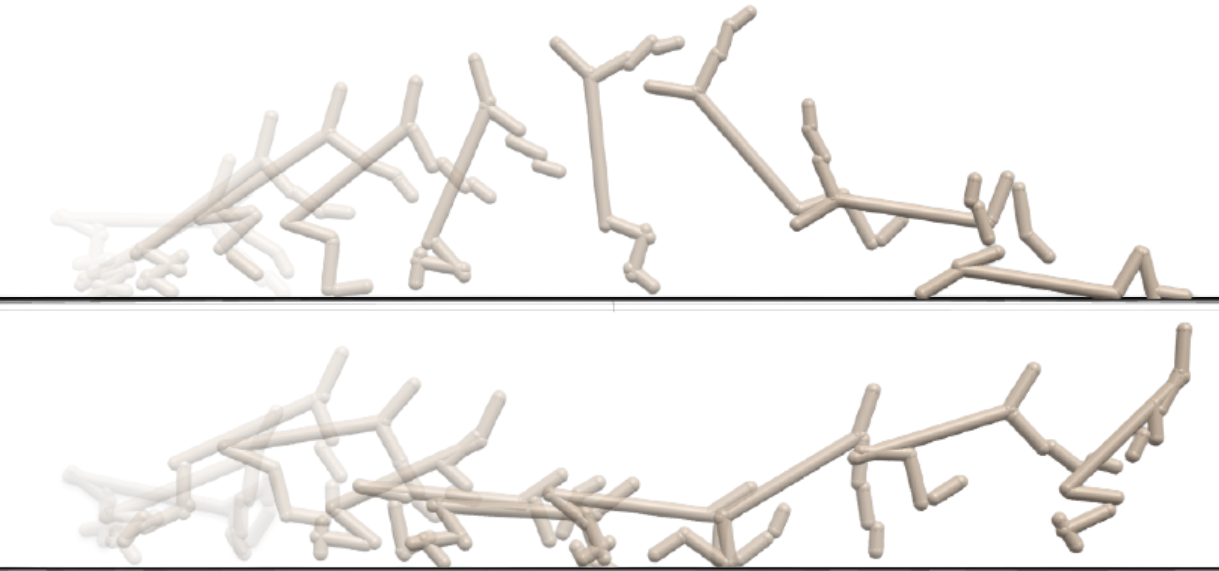
\includegraphics[width=1.0\textwidth]{images/good_bad_cheetah.png}
    %     \vspace{-0.1cm}
    %     \caption{Snapshot of a trajectory on a modified HalfCheetah environment (friction increased by 50\%). On top, PPO fails to generalize. On the bottom, our model LoP adapts quickly and finds an efficient policy after a few shot trials.}
    %      \label{fig:trial}
    % \end{subfigure}
    \vspace{-0.3cm}
    \caption{(Left) An illustration of the process of learning a subspace of policies. (Right) Comparison between PPO and our model in a test environment.}
    \vspace{-0.6cm}
\end{figure}

In this paper, we address a simpler yet harder to tackle generalization setting in which the learning algorithm is trained over one single environment and has to perform well on test environments; preventing us from using meta-RL approaches. A natural way to attack this setting is to start by learning a single policy using any RL algorithm, and to fine-tune this training policy at test time, over the test environment (See red/blue points in Figure \ref{fig:3}), but this process may be costly in terms of environment interactions.

Very recently, the idea of learning a set of diverse yet effective policies  \citep{SMERL,Tokyo} has emerged as a way to deal with this adaptation setting. The intuition is that, if instead of learning one single policy, one learns a set of 'diverse' policies, then there is a chance that at least one of these policies will perform well over a new dynamics. The adaptation in that case just consists in selecting the best policy in that set by evaluating each policy over few episodes (K-shot adaptation).
But the way this set of policies is built and the notion of diversity proposed in these methods have a few drawbacks: these models increase diversity by using an additional intrinsic reward which encourages the different policies to generate different distributions of states. This objective potentially favors the learning of policies that are sub-optimal at train time. Moreover, these approaches make use of an additional component in the policy architecture (e.g., a discriminator) that may be difficult to tune, particularly considering that, at train time, we do not have access to any test environment and thus cannot rely on validation techniques to tune the extra architecture.

%%%est-ce que là on parle de SMERL et DIYAN en disant que c'est une autre façon ou on les ignore
Inspired by recent research on mode connectivity \citep{BentonMLW21,KuditipudiWLZLH19} and by \citep{LearningSubspaces} which aims to learn a subspace of models in the supervised learning setting, we propose to learn a \textbf{subspace of policies} in the parameter space as a solution to the online adaptation in the RL setting (see Figure \ref{fig:3}). Each particular point in this subspace corresponds to specific parameter values, and thus to a particular policy. This subspace is learned by adapting a classical RL algorithm (PPO and A2C in our case, see Section \ref{LoP}) such that an infinite continuum of policies is learned, each policy having different parameters. The policies thus capture and process information differently, and react differently to variations of the training environment (see Figure \ref{fig:k-shot_ant}). 
We validate our approach (Section \ref{sec:res}) over a large set of reinforcement learning environments and compare it with other existing approaches. These experiments show that our method is competitive, achieves good results and does not require the use of any additional component of hyper-parameters tuning contrarily to baselines. 


%Our main contribution is to develop algorithms to learn subspaces of policies in the reinforcement learning setting, and to use these subspaces for online adaptation over unknown test environments. We propose in this paper two concrete algorithms built on top of A2C and PPO for both continuous and discrete actions spaces. This approach is validated over a large set of reinforcement learning environments and compared with other existing approaches, and particularly with approaches based on diversity. These experiments show that our method is competitive and achieve very good results while being sample efficient. We also provide an ablation study to understand the impact of the different components of this model.

